\documentclass{sigchi-ext}
% Please be sure that you have the dependencies (i.e., additional
% LaTeX packages) to compile this example.
\usepackage[T1]{fontenc}
\usepackage{textcomp}
\usepackage[scaled=.92]{helvet} % for proper fonts
\usepackage{graphicx} % for EPS use the graphics package instead
\usepackage{balance}  % for useful for balancing the last columns
\usepackage{booktabs} % for pretty table rules
\usepackage{ccicons}  % for Creative Commons citation icons
\usepackage{ragged2e} % for tighter hyphenation

% Some optional stuff you might like/need.
% \usepackage{marginnote} 
% \usepackage[shortlabels]{enumitem}
% \usepackage{paralist}
% \usepackage[utf8]{inputenc} % for a UTF8 editor only

% Paper metadata (use plain text, for PDF inclusion and later
% re-using, if desired).  Use \emtpyauthor when submitting for review
% so you remain anonymous.
\def\plaintitle{WearLoc: A Wearable Indoor Localization Device} \def\plainauthor{Rick Gelhausen, Jennifer Nist, Lukas Gemein, David Speck
  , Andre Biedenkapp}
\def\emptyauthor{}
\def\plainkeywords{Authors' choice; of terms; separated; by
  semicolons; include commas, within terms only; required.}
\def\plaingeneralterms{Documentation, Standardization}

\title{WearLoc: A Wearable Indoor Localization Device}

\numberofauthors{6}
% Notice how author names are alternately typesetted to appear ordered
% in 2-column format; i.e., the first 4 autors on the first column and
% the other 4 auhors on the second column. Actually, it's up to you to
% strictly adhere to this author notation.
\author{%
  \alignauthor{%
    \textbf{Lukas Gemein}\\
    \email{gemeinl@cs.uni-freiburg.de} }\alignauthor{%
    \textbf{Jennifer Nist}\\
    \email{nistj@cs.uni-freiburg.de} } \vfil \alignauthor{%
    \textbf{Rick Gelhausen}\\
    \email{rick.gelhausen@gmail.com} }\alignauthor{%
    \textbf{David Speck}\\
    \email{speckd@cs.uni-freiburg.de} } \vfil \alignauthor{%
    \textbf{Andre Biedenkapp}\\   
    \email{biedenka@cs.uni-freiburg.de}}} 

% Make sure hyperref comes last of your loaded packages, to give it a
% fighting chance of not being over-written, since its job is to
% redefine many LaTeX commands.
\definecolor{linkColor}{RGB}{6,125,233}
\hypersetup{%
  pdftitle={\plaintitle},
%  pdfauthor={\plainauthor},
  pdfauthor={\emptyauthor},
  pdfkeywords={\plainkeywords},
  bookmarksnumbered,
  pdfstartview={FitH},
  colorlinks,
  citecolor=black,
  filecolor=black,
  linkcolor=black,
  urlcolor=linkColor,
  breaklinks=true,
}

% \reversemarginpar%

\begin{document}

\maketitle

% Uncomment to disable hyphenation (not recommended)
% https://twitter.com/anjirokhan/status/546046683331973120
\RaggedRight{} 

\section{Introduction}
Fire-fighters and other rescue teams often have to roam through burning buildings or tunnels to find and rescue survivors of a tragic event. Thereby they enter unmapped environments and it can be hard not to lose the orientation or to share the location of a survivor to other members of the team. Even if the rescue team has maps of a building, ways can be blocked due to cave-ins. It would be desirable to create maps of the surroundings that are up-to-date. This could make the work for rescue teams easier and safer.\\
Another area of application for such a map generating device would be the mapping of caves, to simplify and secure the work of cave-explorers.\\
There are approaches like hector-SLAM to create live-maps. In the Wearable Computing Systems lab course, we tried two different approaches to create a wearable device running hector-SLAM to create live-maps. The main difference of the approaches lie in the hardware we used. Our first approach was using a raspberry PI and the RPLIDAR to get the system working. In a second step we tried to create a smaller version using an Intel Edison and the Hokuyo laser-scanner.\\
\newpage
\section{Hardware}
In our attempt to create a wearable device we used several hardware components.
\subsection{Raspberry Pi}
The Raspberry PI 2 Model B features a 900MHz quad-core CPU. We use the raspberry pi in our first setup to run the entire software and send the resulting map data to an external device to display the map.
\subsection{Intel Edison}
The Intel Edison features a 500MHz CPU. We use the Intel Edison in our second approach. It is used to run the packages for our IMU and laser-scanner. The laser and IMU data is then send to an external device.
\subsection{Laser-Scanner Robo Peak}
The RPLIDAR is a 360 degree 2D laser-scanner system. The scan range expands from 0.2 to 6m. Due to its huge rotating part and the associate motor, the RPLIDAR is quite big for wearable device, having a surface of about 70x100 $mm^2$. We use it in our first setup mounted on a portable platform.
\subsection{Laser-Scanner Hokuyo}
The Hokuyo laser-scanner has a 240 degree measurement radius. The scan range expands from 0.02 to 4m With its 40x40 $mm^2$ surface it is ideal to be mounted on a GoPro holder, which allows hundreds of different possible wearable designs.
\subsection{Grove-IMU}
The Grove-IMU 9DOF v2.0 features a gyroscope, a magnetometer and a accelerometer. We use the Grove-IMU in both our setups to measure the bearing of the laser-scanners to track the users rotation. Furthermore it helps to better predict our location.
\section{Software}
Our entire project is based on the ROS package for hector-SLAM created by a team of the University of Darmstadt. We run a ROS-core on a laptop, together with the hector-slam package. The packages required for reading the data from the sensors run on the Intel Edison. In our first attempt using the Raspberry PI we ran everything on the Raspberry and transferred the map data to a laptop. Now we send the data from the sensors to the laptop and build the map there. 
\section{Approach 1}
In our first approach, we used the Raspberry PI, the Grove-IMU and the RPLIDAR. We chose to work on this approach because we waited for our circuit board for the Intel Edison to be finished. This allowed us to get familiar with the hardware and the hector-SLAM packages for ROS. The Raspberry PI is very user-friendly and allowed a fast entry into the topic.\\
In this approach the ROS packages for the individual hardware parts, together with hector-SLAM, run on the Raspberry PI. The map data is then send to a external device, like a laptop, via Wifi.\\ 
As we are trying to create a wearable device, the disadvantage of this approach is the size of the Raspberry PI and the RP Lidar.
\section{Approach 2}
In our second approach, we use the Intel Edison, the Grove-IMU and both the Hokuyo laser-scanner and the RP Lidar.\\
In this approach the ROS packages for the laser-scanner and the IMU run on the Intel Edison and the data is send to a laptop via Wifi. In this case hector-SLAM runs on the laptop.\\
In comparison to the the first approach, this is very compact.
We created two major setups, one using the Hokuyo laser-scanner and one using the RP Lidar. The Hokuyo laser-scanner is small enough to be mounted on a platform that can be attached to GoPro-Camera holders. The IMU is then attached to the bottom of the platform. As there is an enormous amout of different GoPro-Camera holders, this allows us to attach the laser-scanner and the IMU in many different ways. One way would be to attach the Scanner on a helmet, like a helmet lamp. Like this both hands are free for other tasks.\\
Another setup we created using the RP Lidar, is a portable platform on which all the necessary hardware is mounted. In comparison the the other setup, this is very stable but need one hand to hold the platform.\\
%TODO ADD PICTURES OF BOTH SETUPS
%\begin{figure}
%  \includegraphics[width=0.9\columnwidth]{}
%  \caption{Insert a caption below each figure.}~\label{fig:sample}
%\end{figure}
\section{Results}
We managed to obtain satisfying results using our second approach. We noticed that, even though the resolution of the Hokuyo laser-scanner is better than the resolution of the RP lidar, we have better results using the RP lidar. The disadvantage of the Hokuyo is the limited range of maximum 4 meters. The RP lidar has a range of 5.5 meters and therefore returns more reference points to estimate its location. Using a laser-scanner with even higher range, we could significantly improve our results.
\begin{figure}
	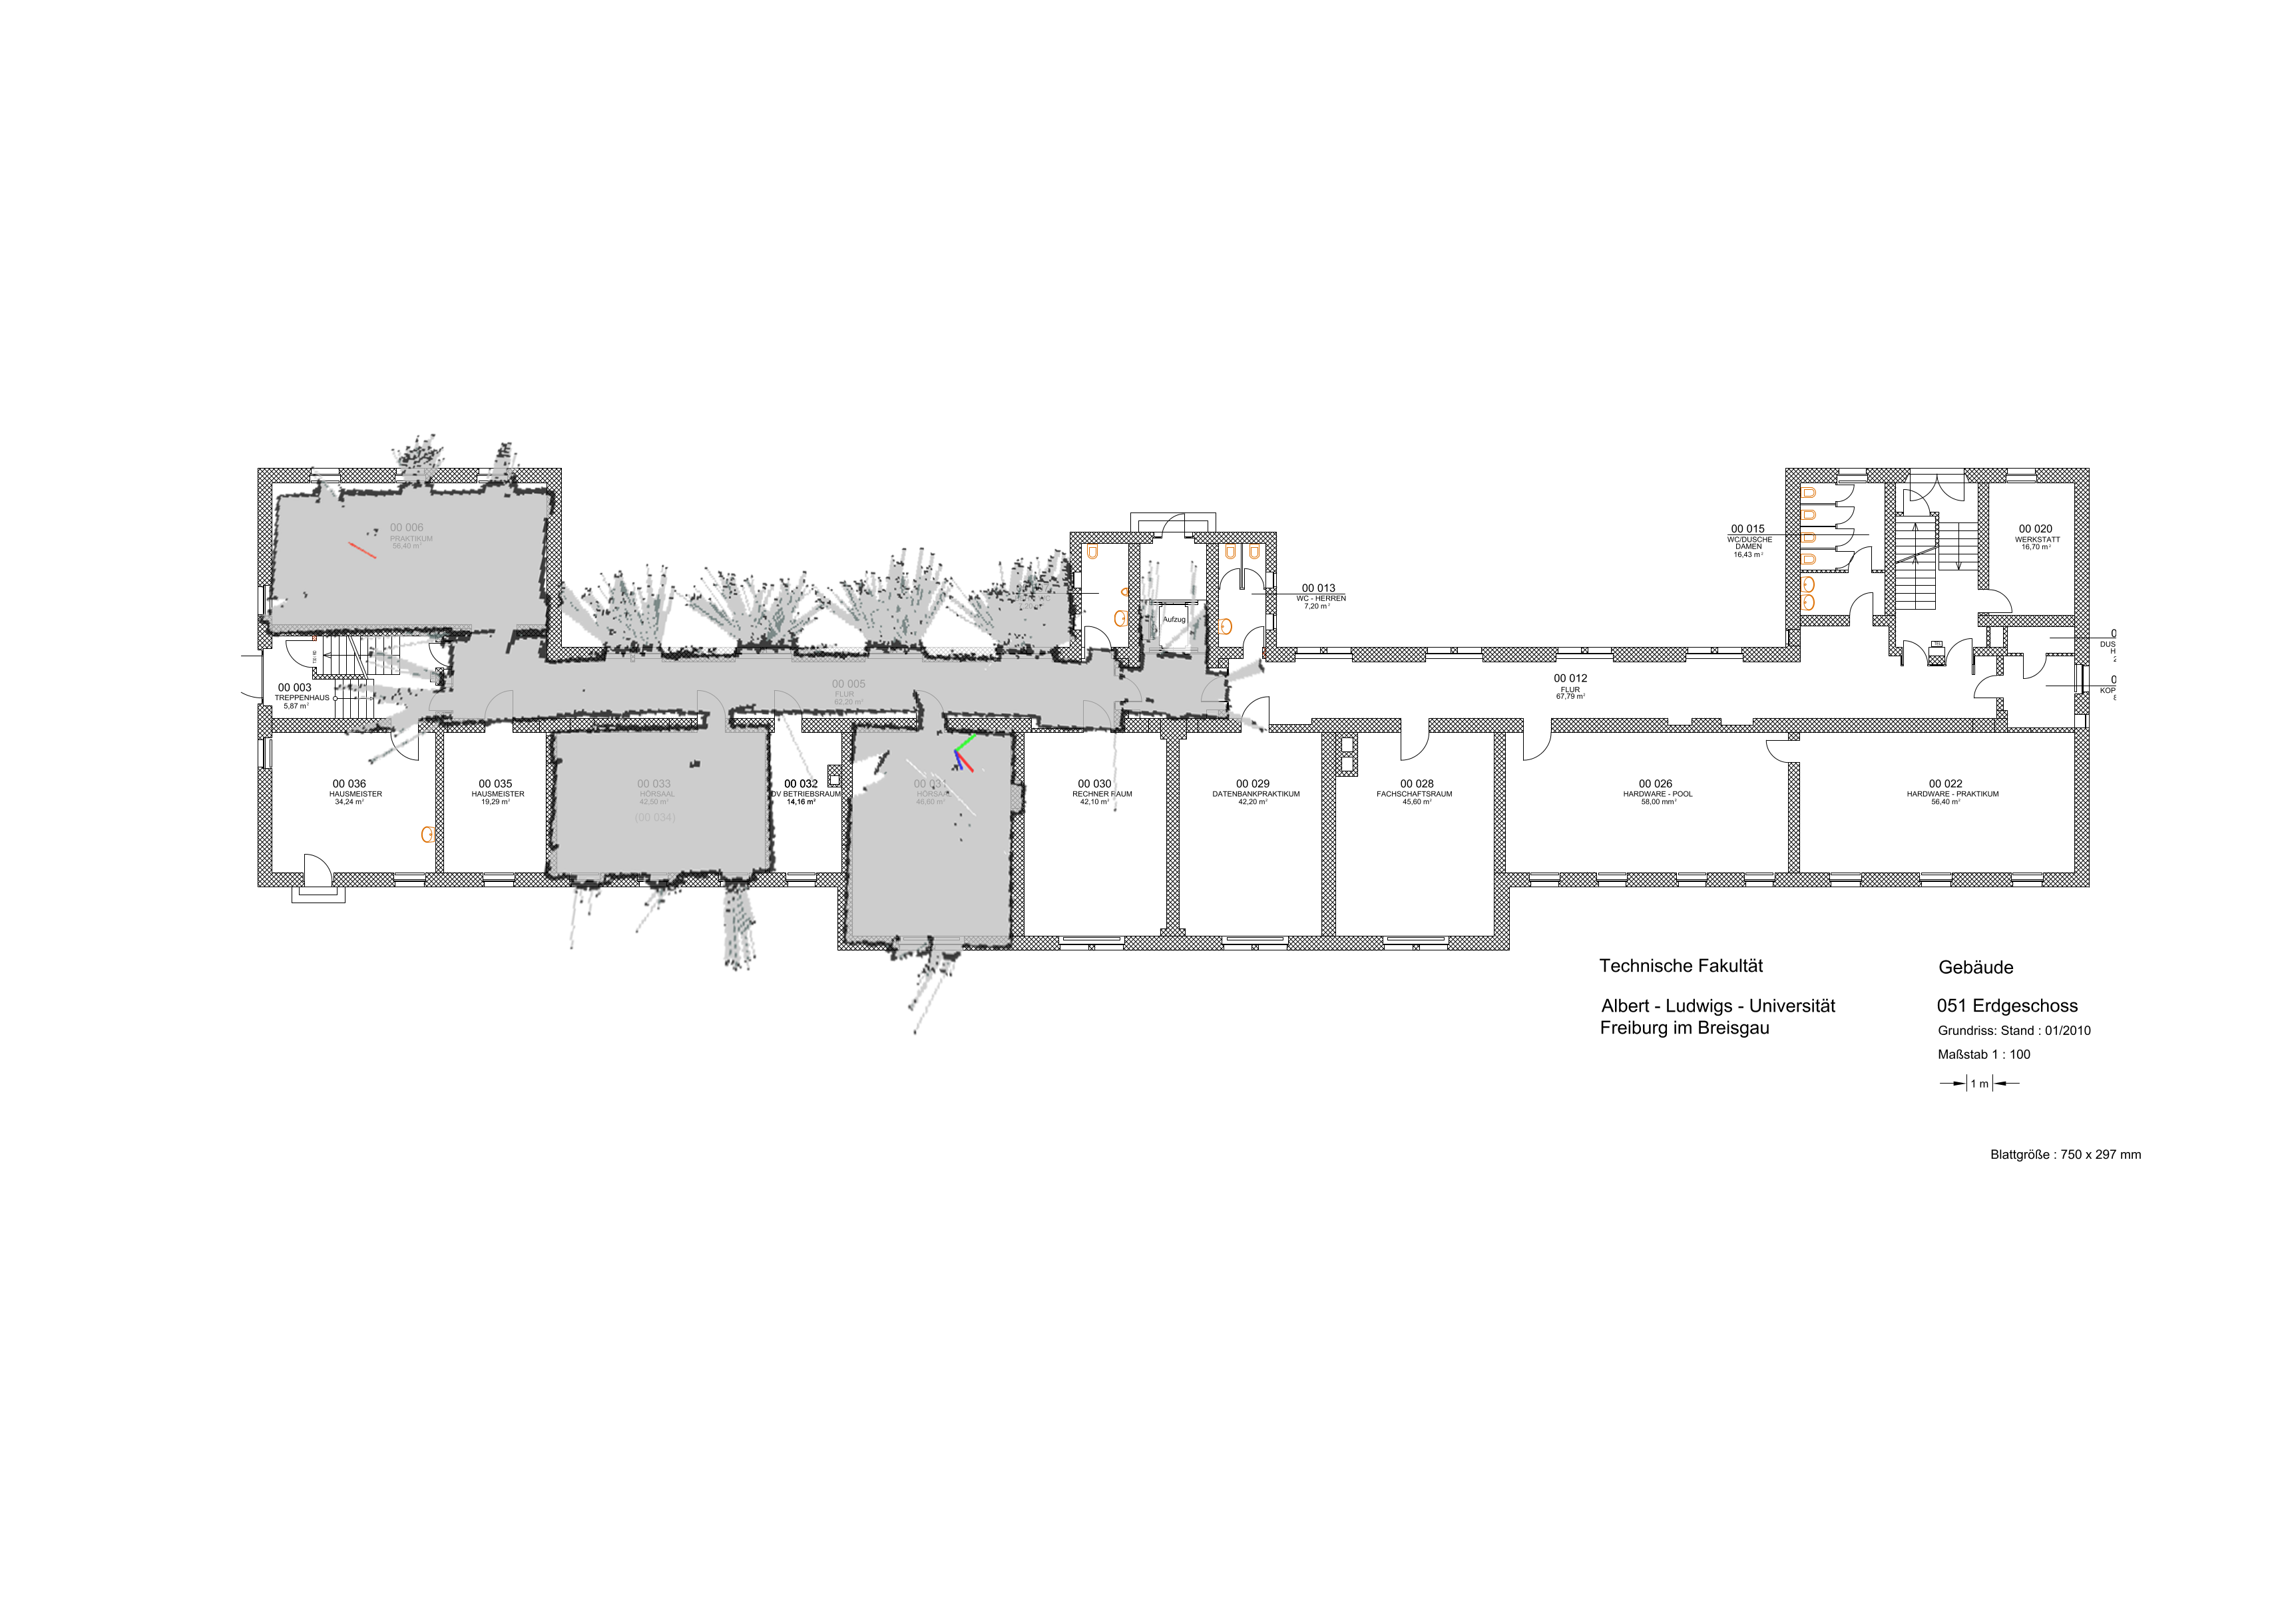
\includegraphics[width=0.9\columnwidth]{51.png}
	\caption{University of Freiburg. Mapped overlay of Building 51}~\label{fig:sample}
\end{figure}
%\bibliographystyle{SIGCHI-Reference-Format}
%\bibliography{sample}

\balance{} 
\end{document}